 
\chapter{Pipeline}
El pipelining es una técnica de implementación donde múltiples instrucciones son solapadas en ejecución; toma ventaja del paralelismo que existe entre las acciones requeridas para ejecutar una instrucción.

Un pipeline es como una línea de ensamblado. Por ejemplo, en una línea de ensamblado automotriz, hay muchas etapas, cada una contribuye a la construcción del auto. Cada una opera en paralelo de las otras para diferentes autos. En el pipeline de una computadora, cada etapa completa una parte de la instrucción.

Se define el \textit{throughput} en una línea de ensamblado de autos como el número de autos por hora y se determina por que tan seguido se termina un auto en la línea de montaje. En las computadoras, esto es análogo, y se determina por que tan seguido se completa una instrucción en el pipeline.

Esta técnica de pipelining reduce el tiempo de ejecución promedio por instrucción. Dependiendo de que se considera como base, esta reducción puede ser vista como una reducción en el número de ciclos de reloj por instrucción (CPI) o como una reducción en el tiempo del ciclo de clock o como una combinación. Si se considera un procesador que toma múltiples ciclos de clock por instrucción, entonces pipelining es usualmente visto como una reducción del CPI.

Cada instrucción RISC puede ser implementada como mucho en 5 ciclos de reloj.

\begin{center}
 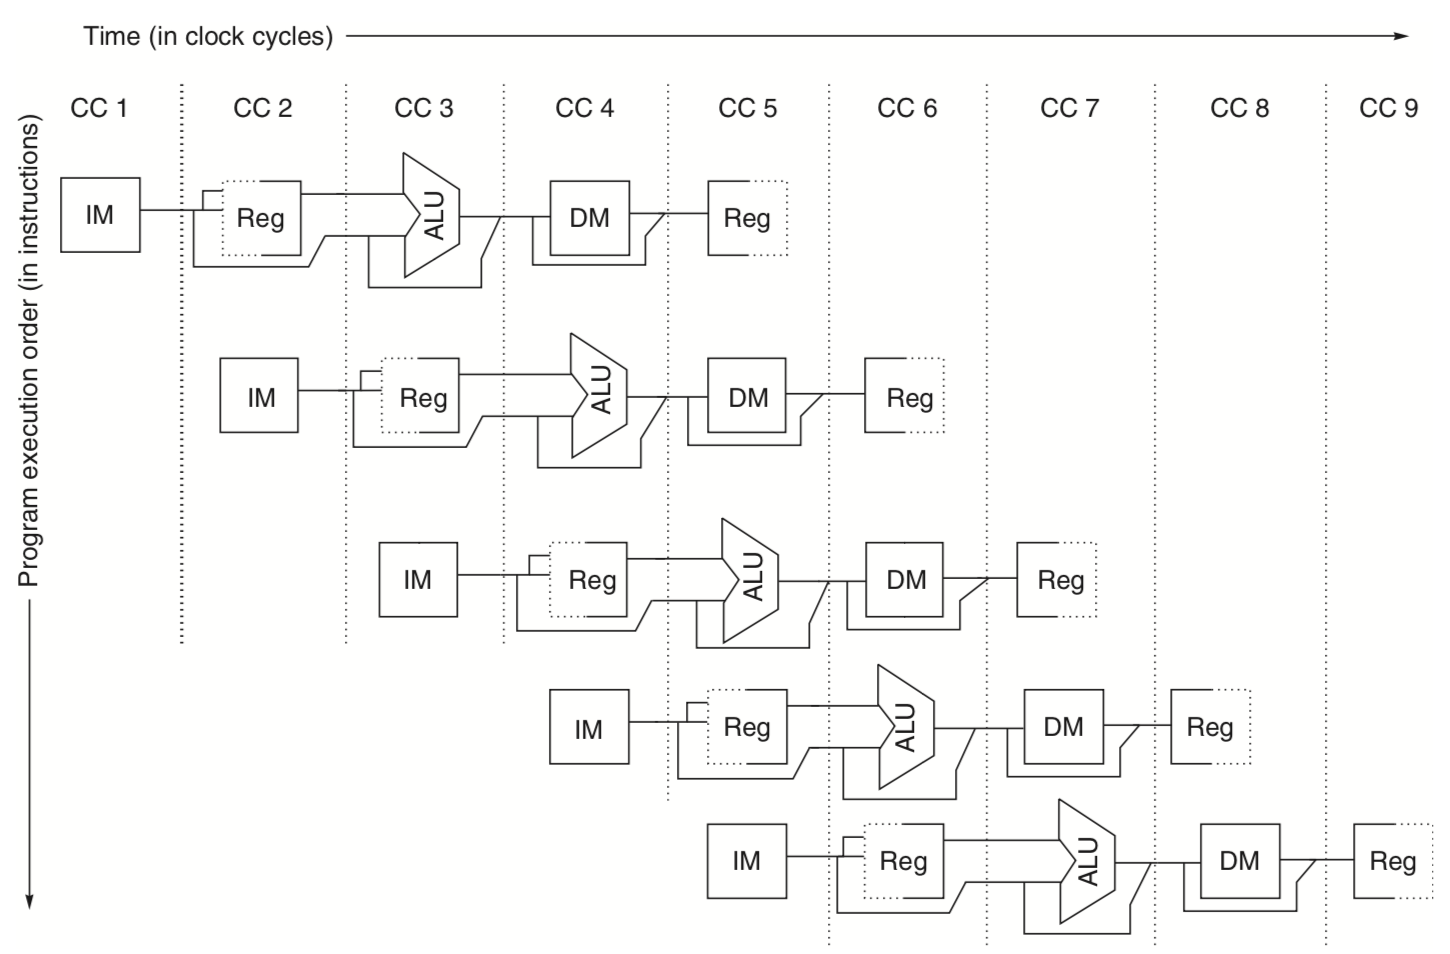
\includegraphics[scale=.5,keepaspectratio=true]{gfx/pipeline2.png}
\end{center}


\begin{enumerate}
 \item Instruction fetch cycle (IF):
 
Se manda el program counter (PC) a memoria y trae la instrucción actual de memoria. Se actualiza el PC para la próxima instrucción secuencial sumando 4 dado que cada instrucción es de cuatro bytes.

\item Instruction decode/register fetch cycle (ID):

Se decodifica la instrucción y se leen los registros especificados del register file. Se verifica la igualdad mientras se leen los registros por un posible branch. Se extiende el signo en caso de ser necesario y se calcula la dirección destino del salto sumando el offset de la extensión de signo al PC.

\item Execution/effective address cycle (EX):

La ALU ejecuta en los operandos dependiendo el tipo de instrucción:

\begin{itemize}
 \item Referencia a memoria. La ALU suma al registro base el offset para formar la dirección efectiva.
 \item Registro - Registro. La ALU realiza la operación especificada en el opcode sobre los valores leídos del register file.
 \item Registro - Inmediato. La ALU realiza la operación especificada en el opcode sobre el primer valor leído del register file y el inmediato con signo extendido.
\end{itemize}

\item Memory access (MEM):

Si la instrucción es un load, se hace una lectura a memoria usando la dirección efectiva calculada en el ciclo anterior. Si es un store, se escribe a memoria el dato del segundo registro leído del register file usando la dirección efectiva.

\item Write Back cycle (WB):

Escribe el resultado en el register file, ya sea que viene de memoria (load) o de la ALU. 
\end{enumerate}

En esta implementación, las instrucciones de salto requieren dos ciclos, las instrucciones de store requieren 4 y todas las demás 5 ciclos.

\begin{center}
 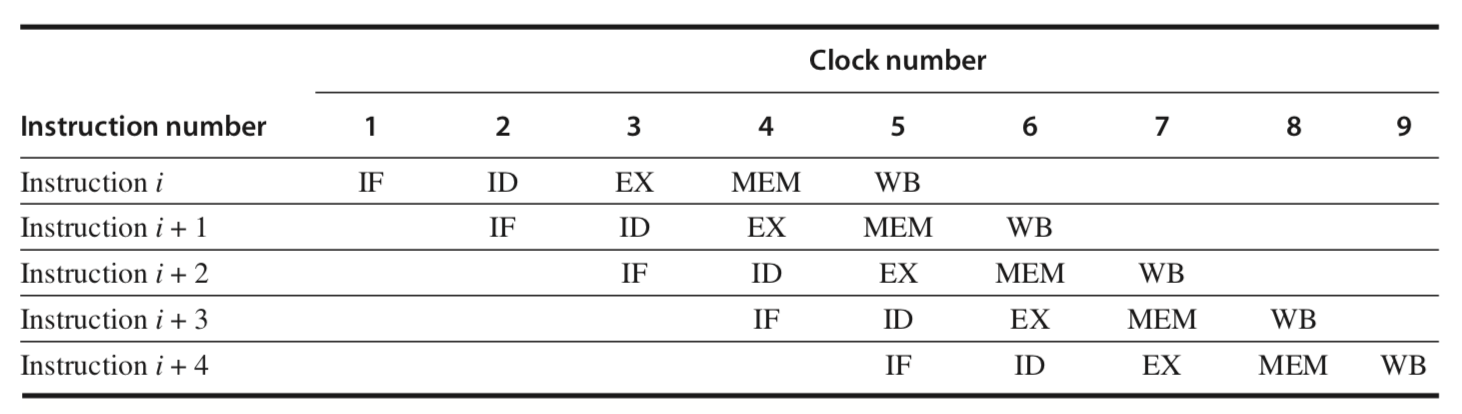
\includegraphics[scale=.55,keepaspectratio=true]{gfx/pipeline1.png}
\end{center}


\section{Pipeline Hazards}
Los riesgos (hazards) en el pipeline se pueden clasificar de tres formas:

\begin{enumerate}
 \item Estructurales. Estos hazards ocurren por conflicto de recursos cuando el hardware no puede soportar todas las combinaciones posibles de instrucciones simultáneamente.
 \item De datos. Ocurren cuando una instrucción depende del resultado de una instrucción previa de forma que se solapan en el pipeline.
 \item De control. Ocurren por los saltos y otras instrucciones que modifican al PC.
\end{enumerate}

\section{Data Hazards}
\subsection{Minimizando los Hazards de datos con forwarding}

La técnica de forwarding funciona de la siguiente manera:

\begin{enumerate}
 \item El resultado de la ALU ya sea de la etapa EX/MEM o MEM/WB se conecta de vuelta a las entradas de la ALU.
 \item Si el hardware de forwarding detecta que la operación previa de la ALU ha escrito al registro correspondiente como fuente de la operación actual, se toma el resultado de las entradas de la ALU en vez del valor leído del register file.
\end{enumerate}
 

Por ejemplo en la siguiente secuencia de instrucciones, no es posible aplicar forwarding.

\begin{verbatim}
 LD     R1,0(R2) 
 DSUB   R4,R1,R5 
 AND    R6,R1,R7 
 OR     R8,R1,R9
\end{verbatim}


\section{Branch Hazards}

Recordar que si un salto cambia al PC a la dirección target, el salto es tomado, si continua, entonces, es no tomado. Cuando la instrucción siguiente es de un salto tomado, en realidad, el PC no se modifica hasta el final de la etapa de ID.

El esquema más simple para manejar los saltos es freezar o vaciar el pipeline, manteniendo o eliminando las instrucciones después del salto hasta conocer el destino. En este caso, la penalidad de salto es fija y no puede minimizarse por software.

Otro esquema apenas más complejo es tratar cada salto como no tomado y dejar que se continúe como si el salto no se ejecutase. La precaución que hay que tener en cuenta es no cambiar el estado del procesador hasta que se conozca realmente la salida del salto. 

\begin{center}
 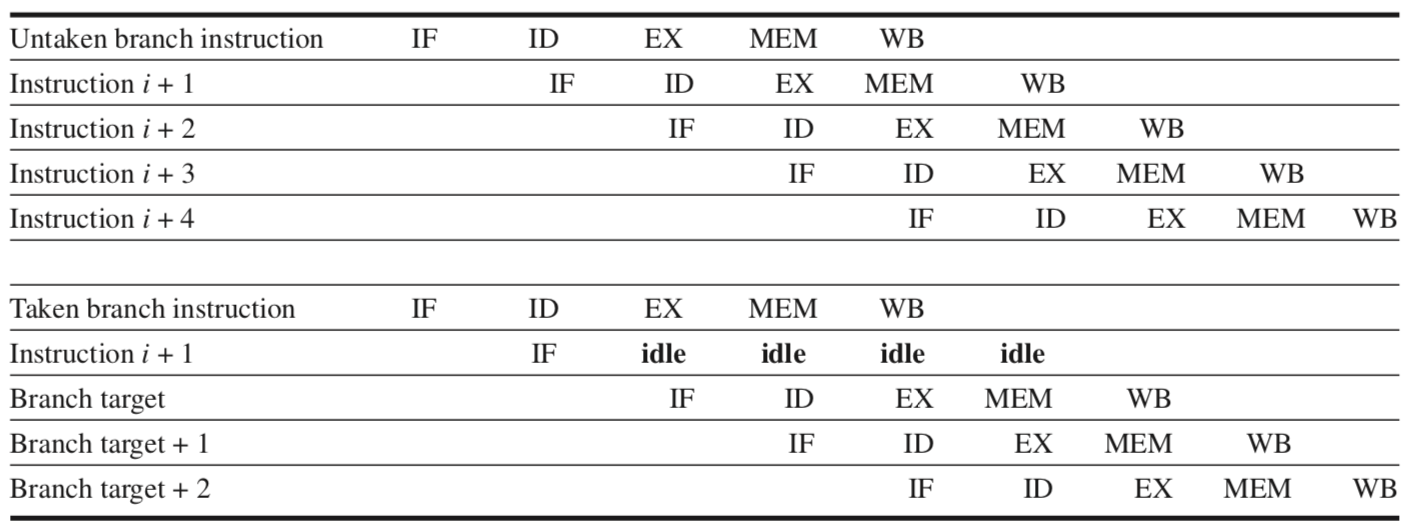
\includegraphics[scale=.5,keepaspectratio=true]{gfx/pipeline0.png}
\end{center}

Si el salto es tomado, hay que cambiar la instrucción que se hizo el fetch y convertirá a no-op y reiniciar el fetch a la dirección target.


Otro esquema para lidiar con los salto es el del salto demorado,

\begin{verbatim}
 branch  instruction
 sequential   successor
 branch target if taken
\end{verbatim}

La secuencia elegida se coloca en el branch delay slot. Esta instrucción es ejecutada de todas formas se tome o no se tome el salto.


\begin{center}
 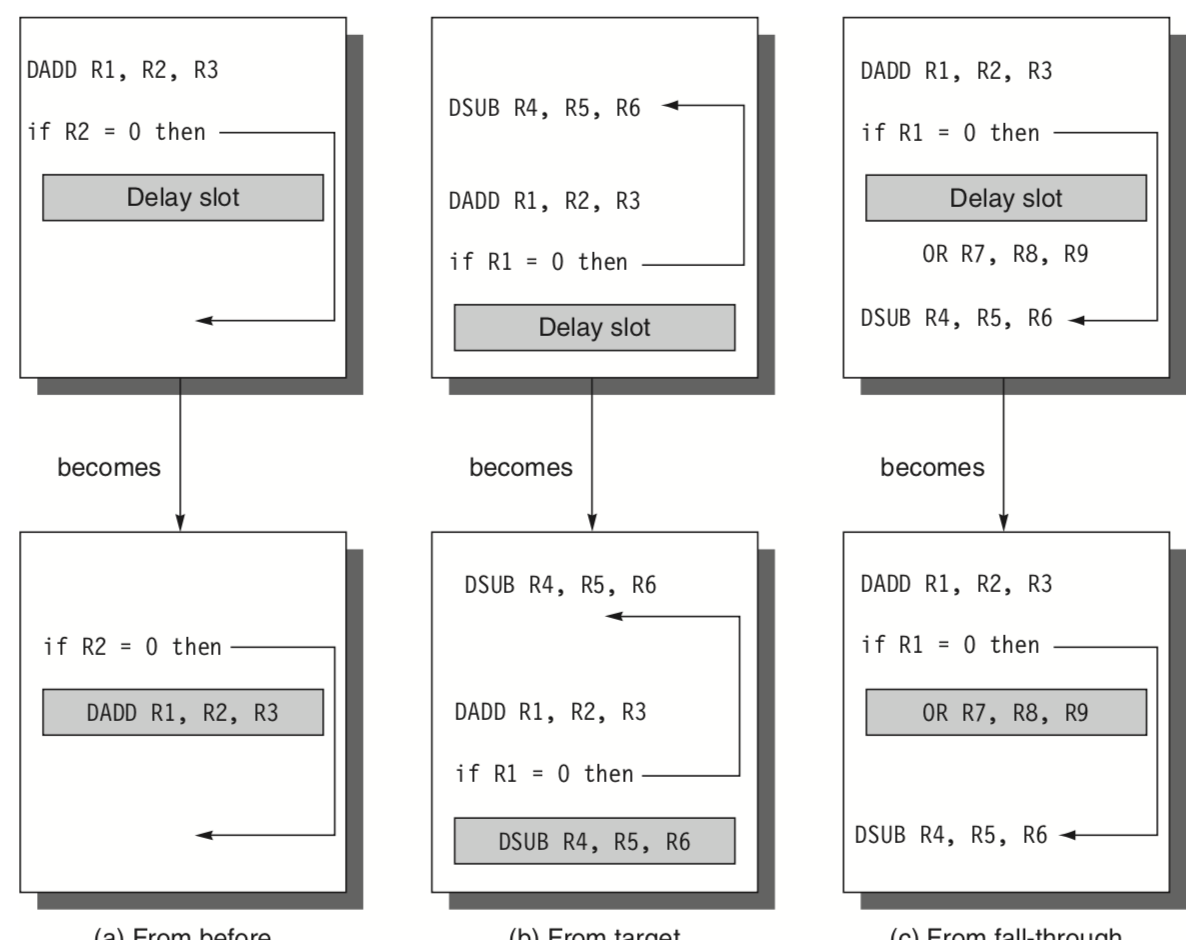
\includegraphics[scale=.5,keepaspectratio=true]{gfx/static_branch.png}
\end{center}



\subsection{Dynamic Branch Prediction y Branch-Prediction Buffers} 
Un branch-prediction buffer es una memoria pequeña indexada por la parte mas baja de la dirección de la instrucción de salto. Esta memoria contiene un bit que indica si el salto fue recientemente tomado o no. 
 
Este buffer efectivamente es una cache donde cada acceso es un hit y la performance depende de la predicción del salto y que tan bien se predijo.

El esquema de predicción de un bit no tiene tan buena performance ya que incluso si el salto siempre se toma se estaría prediciendo dos veces en forma incorrecta en lugar de una, cuando el salto no se toma el haber errado provoca que el bit se cambie.
 
Para solucionar este inconveniente se utiliza un esquema de 2-bit donde hay que predecir mal dos veces para cambiar la decisión.
 

\begin{center}
 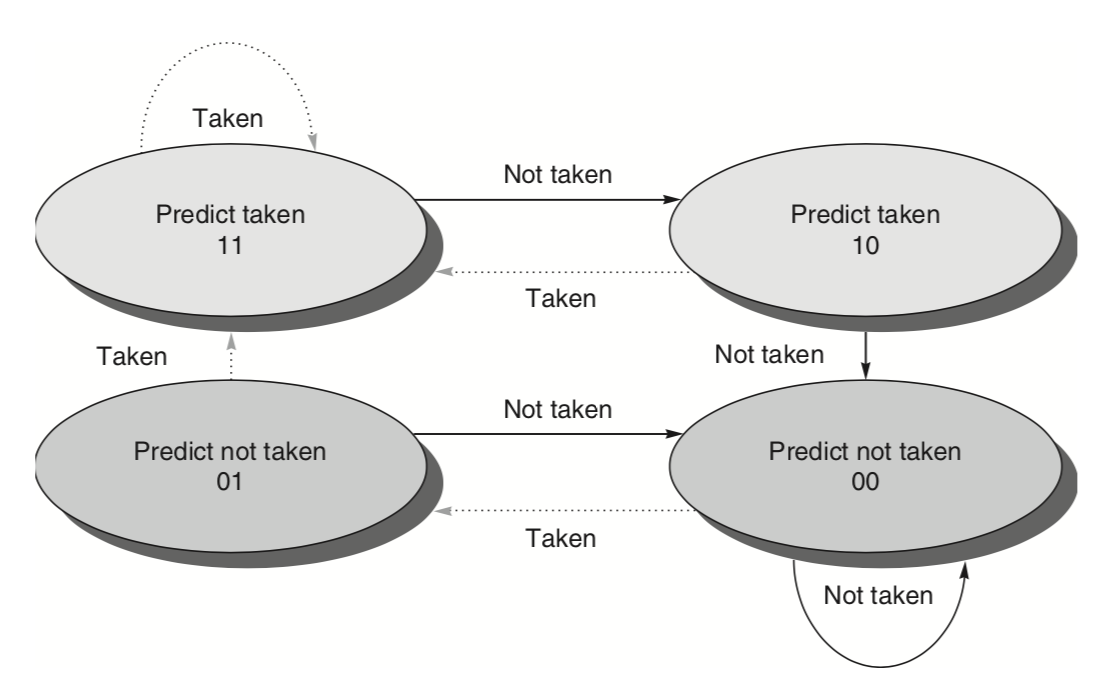
\includegraphics[scale=.5,keepaspectratio=true]{gfx/branch_prediction.png}
\end{center}

